\section{Розширення маски хмар}

Для уточнення маски хмар був використаний алгоритм Dilation.

Розширення (Dilation) - один з двох основних операторів
математичної морфології, інший - ерозія. Зазвичай він застосовується до
двійкових зображень, але є версії, які працюють на зображеннях grayscale
зображень. Основний ефект оператора на бінарне зображення полягає в
поступовому збільшенні меж областей пікселів переднього плану. Таким
чином, ділянки пікселів переднього плану збільшуються в розмірі, тоді як
отвори в цих регіонах стають меншими.

Розширення бінарної множини $A$ структурним %
елементом $B$ визначають як \begin{equation}
  A \oplus B = \{s \mid \widehat{B}_s \cap A \ne \varnothing\}.  \label{eq:dilation-set}
\end{equation}

Якщо зображення це $f(x)$, а структурний елемент $b(x)$, тоді розширення
$f$ на $b$ визначається формулою \ref{eq:dilation-grayscale}:
\begin{equation}
(f \oplus b)(x) = \sup_{y \in E} [f(y) + b(x - y)] \label{eq:dilation-grayscale}
\end{equation}

При використанні великих структурних елементів $b(x)$ формується за
формулою \ref{eq:dilation-structuring-element}:
\begin{equation}
b(x) = \begin{cases}
0, & x \in B, \\
-\infty, & \text{інакше}
\end{cases} \label{eq:dilation-structuring-element}
\end{equation}

де $B$ є підмножиною $\mathbb{R} \cup \{-\infty, +\infty\}$

У такому випадку розширення будується за формулою
\ref{eq:dilation-supremum}:
\begin{equation}
(f \oplus b)(x) = \sup_{z \in E} [f(x - z) + b(z)] = \sup_{z \in B} [f(x - z)] \label{eq:dilation-supremum}
\end{equation}

\begin{figure}[H]
    \centering
    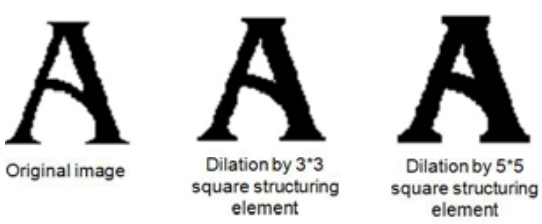
\includegraphics[width=0.6\textwidth]{images/image6}
    \caption{Приклад застосування оператора розширення
        \label{fig:operator_dilation_example}
    }
\end{figure}

Сам процес розширення (рис. \ref{fig:operator_dilation_example}) є не складним:
нехай є певна множина, яка потребує збільшення або розширення, тоді існує ще одна
множина, яка виступає у ролі структурного елемента. Тоді структурний
елемент проходиться по межах розширюючої множини і збільшує її границі
на заданий розмір. Таким чином, ми одержуємо множину, що має ту ж саму
форму, що й оригінальна, але вже збільшена.


Розглянемо приклад застосування оператора розширення
у випадку супутникових даних, а саме окремого композиту та його маски.


З цього знімка (рис. \ref{fig:example_cloud}) був зроблений композит та
взята його маска (рис. \ref{fig:cloud-mask-a}). З маски було витягнуто окремі пікселі, що
відповідають окремо за перисті хмари та самі хмари. Тобто взято {10} та
{2,3,8,9} значення пікселів відповідно та розширено (рис. \ref{fig:dilated-cloud-mask-b}) за
допомогою оператора.

\begin{figure}[H]
    \centering
    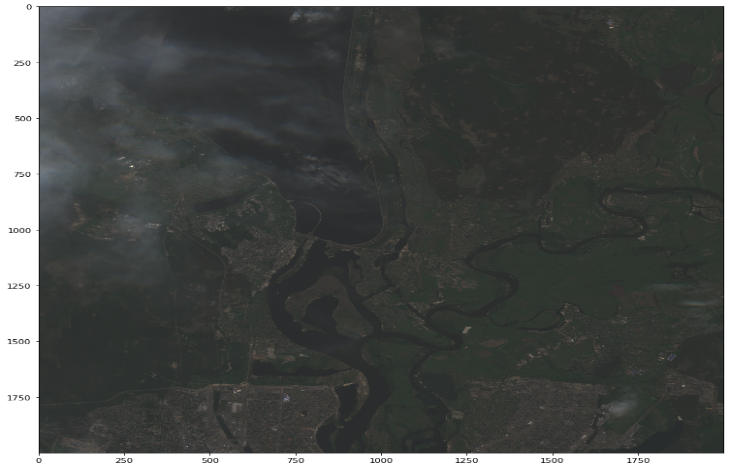
\includegraphics[width=0.7\textwidth]{images/image7}
    \caption{Знімок зроблений 2019-06-07 розміром 2000х2000
        \label{fig:example_cloud}
    }
\end{figure}

\begin{figure}[H]
  \centering \subfloat[Маска хмар]{
    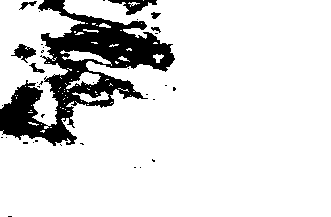
\includegraphics[width=0.35\textwidth,height=0.2\textheight]{images/image8}
    \label{fig:cloud-mask-a}
  } \subfloat[Розширена маска хмар]{
    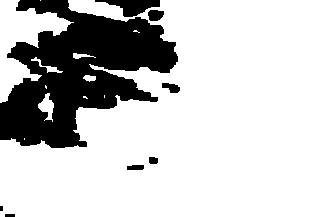
\includegraphics[width=0.35\textwidth,height=0.2\textheight]{images/image9}
    \label{fig:dilated-cloud-mask-b}
  } \caption{Маски хмар до та після розширення}
\end{figure}
